\documentclass[]{beamer}
\usepackage[T1]{fontenc}
\usepackage[utf8]{inputenc}
\usepackage{lmodern}
\usepackage[italian]{babel}
\usepackage{multicol}
\usepackage{cancel}

\title{Temperatura e calore}
\author{\texorpdfstring{Mattia Cozzi\newline\href{mailto:cozzimattia@gmail.com}{\texttt{cozzimattia@gmail.com}}}{Mattia Cozzi}}
\date{a.s.~2023/2024}

%\documentclass[handout]{beamer}     %usare questa classe per generare l'handout
%\usepackage{pgfpages}   %per mostrare più quadri nella stessa pagina
%\pgfpagesuselayout{4 on 1}[a4paper,border shrink=5mm,landscape]
\usetheme{Singapore}
%\useoutertheme[left]{sidebar} %elementi intorno alle diapositive
\setbeamercovered{dynamic} %modifica l'aspetto del testo grigetto delle diapositive future. Argomenti: invisible/transparent/dynamic
\usecolortheme{orchid}
%COLORE PRINCIPALE
% \definecolor{marroncino}{RGB}{156, 26, 0} % UBC Blue (primary)
% \setbeamercolor{structure}{fg=marroncino} % itemize, enumerate, etc

\theoremstyle{plain}
\newtheorem{teorema}{Teorema}

\usepackage{tikz}


\usepackage{pgf,pgfplots,graphicx}
\usetikzlibrary{angles,quotes,arrows,shapes,decorations.markings}
\pgfplotsset{compat=1.15}
\usepgfplotslibrary{units,fillbetween} % to add units easily to axis
\tikzset{fleche/.style args={#1:#2}{postaction=decorate,decoration={name=markings,mark=at position #1 with {\arrow[#2,scale=2]{>}}},},}



\begin{document}

\begin{frame}
  \titlepage
\end{frame}





\begin{frame}
\frametitle{Contenuti}
\tableofcontents
\end{frame}


\section{Dilatazione}


\begin{frame}
\frametitle{Scale di temperatura}
Misureremo la temperatura di un corpo in:
\begin{itemize}
  \item \alert<1>{gradi celsius ($ ^\circ C $)}, scala relativa al punto di ebollizione e solidificazione dell'acqua;\pause
  \item \alert<2>{kelvin ($ K $)}, scala assoluta (non dipende dall'acqua!).\pause
\end{itemize}

~

Attenzione:
\begin{itemize}
  \item la variazione di $ 1 \, K $ è identica alla variazione di $ 1 \, ^\circ C $;
  \begin{center}
  $ \Delta T_{^\circ C} = \Delta T_K $
  \end{center}
  \pause
  \item lo zero kelvin (zero assoluto, cioè la minima temperatura raggiungibile) si trova a $ -273,15 \, ^\circ C $.
  \begin{center}
  $ T_K = T_{^\circ C} + 273,15 \, K $
  \end{center}
\end{itemize}
\end{frame}



\begin{frame}
\frametitle{Dilatazione lineare dei solidi}
I corpi solidi, se riscaldati, tendono a dilatarsi (a causa della maggiore agitazione termica degli atomi) e \alert{la dilatazione è direttamente proporzionale alla variazione di temperatura}.\pause

~

Per \emph{corpi estesi in una dimensione} vale la legge:
\begin{center}
\colorbox{blue!30}{$ \Delta \ell = \ell_0 \lambda \Delta T  $}
\end{center}
  \begin{multicols}{2}
$ \ell_0 = $ lunghezza iniziale $ [m] $

~

$ \Delta \ell = $ variaz.~di lunghezza $ [m] $

~

$ \lambda = $ coefficiente $ [K^{-1}] $ o $ [^\circ C^{-1}] $

~

$ \Delta T = $ var.~di temperatura \\~~~~~~~~ $ [K] $ o $ [ ^\circ C] $
  \end{multicols}
\end{frame}





\begin{frame}
\frametitle{Esempi}
\begin{columns}
\begin{column}{0.3\textwidth}
\begin{figure}
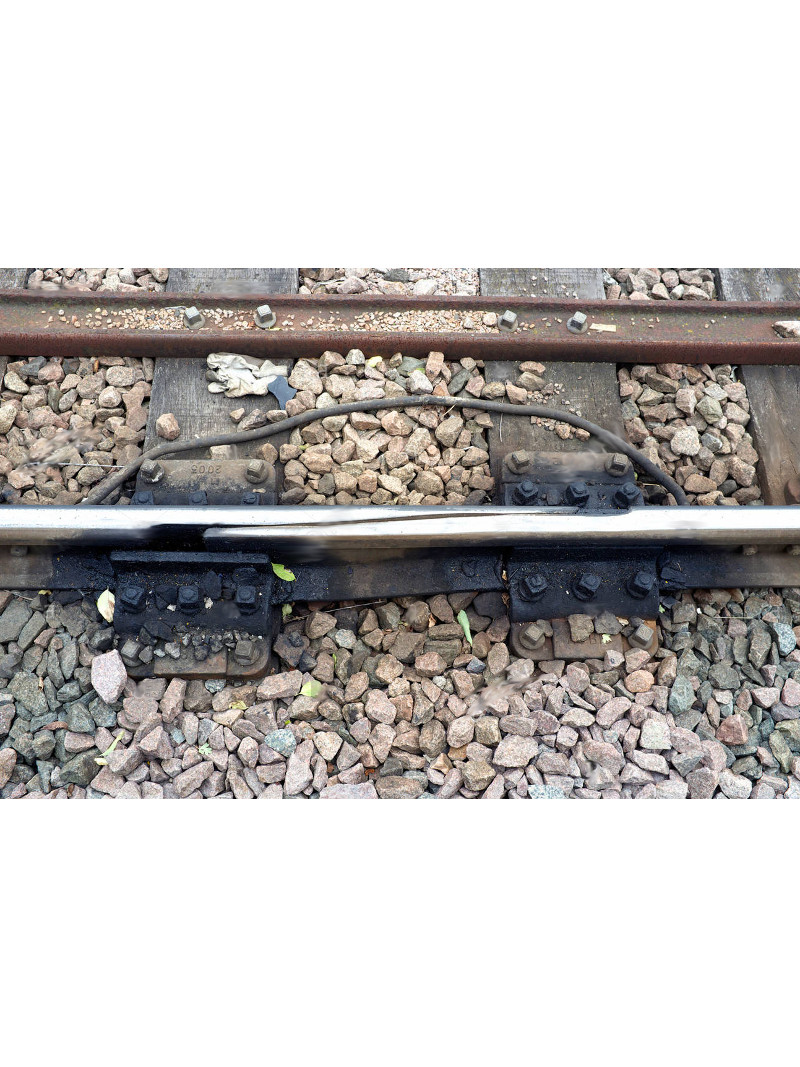
\includegraphics[width=\columnwidth]{img/binari.jpg}
\end{figure}
Giunti di dilatazione su dei binari
\end{column}
\begin{column}{0.3\textwidth}
\visible<2-3>{\begin{figure}
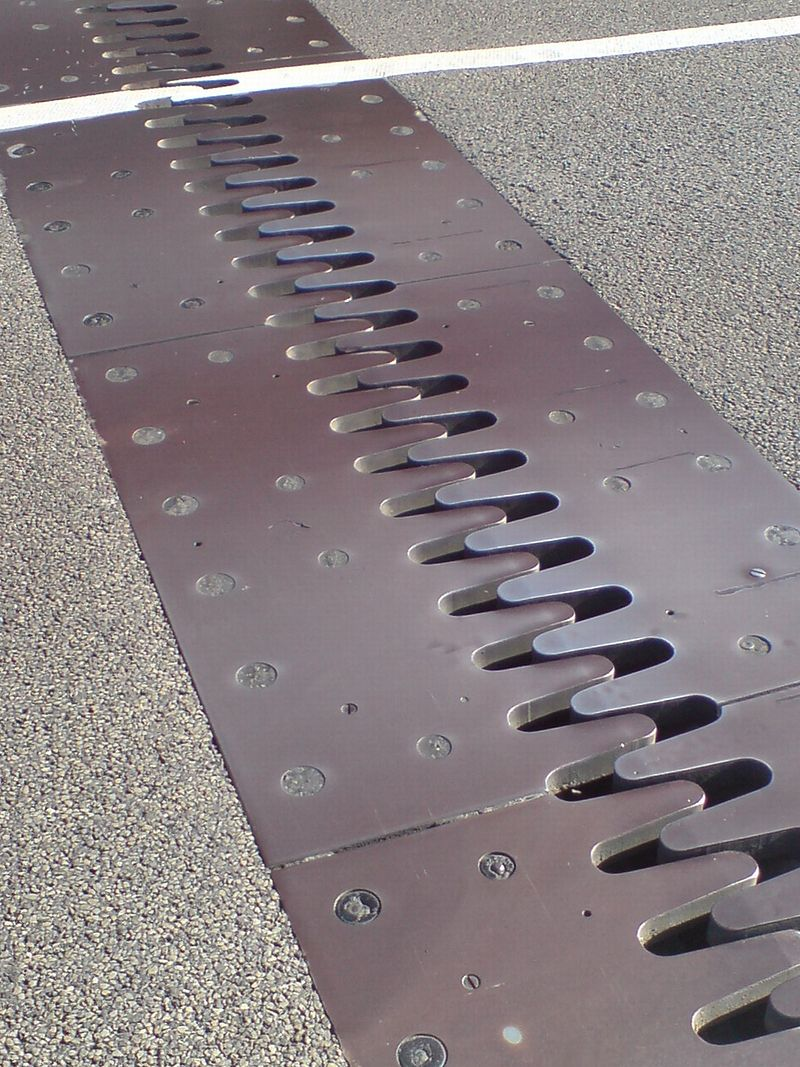
\includegraphics[width=\columnwidth]{img/ponte.jpg}
\end{figure}
Giunti di dilatazione su un ponte}
\end{column}
\begin{column}{0.3\textwidth}
\visible<3>{\begin{figure}
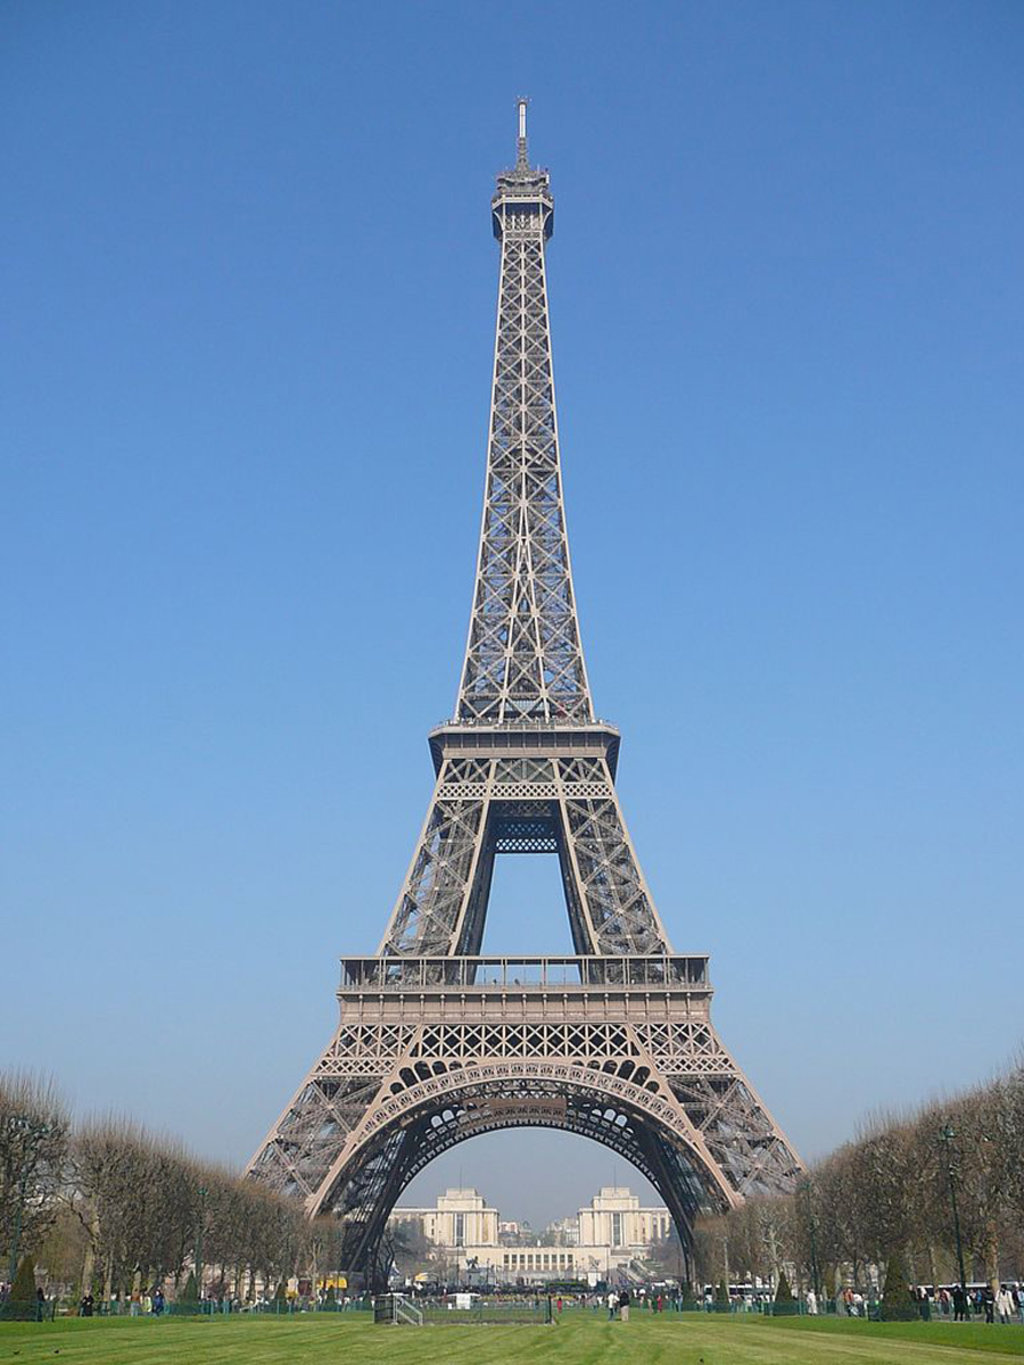
\includegraphics[width=\columnwidth]{img/eiffel.jpg}
\end{figure}
Tour Eiffel ($ 324 \, m $): in estate, $ +15 \, cm $}
\end{column}
\end{columns}
\end{frame}




\begin{frame}
\frametitle{Esempio}
\begin{exampleblock}{Calcolo del coefficiente di dilatazione}
{\small Un filo di ottone di lunghezza iniziale $ \ell_0 = 1,60 \, m $ si allunga della quantità $ \Delta\ell = 4,7 \, mm $ quando viene riscaldato di $ \Delta T = 140 \, K $.
\begin{itemize}
  \item Calcola il coefficiente di dilatazione lineare $ \lambda $ dell'ottone.
\end{itemize}}
\end{exampleblock}\pause

~

Partiamo ora da $ \Delta \ell = \ell_0 \lambda \Delta T $ e invertiamo la formula:
\begin{center}
$ \lambda = \dfrac{\Delta\ell}{\ell_0 \Delta T} $
\end{center}\pause

Convertiamo le misure in notazione scientifica e calcoliamo:
\begin{center}
$ \lambda = \dfrac{4,7 \times 10^{-3}\, m}{(1,60 \, m)\cdot(1,40 \times 10^2 \, K)} =\pause 2,1 \times10^{-5} \, \dfrac{1}{K} $
\end{center}
\end{frame}



\begin{frame}
\frametitle{Lunghezza finale}
Calcoliamo la lunghezza finale dell'oggetto:
\begin{center}
$ \ell_1 = \ell_0 + \Delta \ell $

~

$ \ell_1 = \ell_0 + \ell_0 \lambda \Delta T $

~

\colorbox{blue!30}{$ \ell_1 = \ell_0 ( 1 + \lambda \Delta T ) $}
\end{center}
\end{frame}



\begin{frame}
\frametitle{Dilatazione volumica}
\begin{columns}
\begin{column}{0.65\textwidth}
Per corpi egualmente estesi nelle tre dimensioni valgono leggi analoghe, relative al \alert{volume del corpo}:
\begin{center}
\colorbox{blue!30}{$ \Delta V = V_0 \alpha \Delta T $}

~

\colorbox{blue!30}{$ V_1 = V_0 ( 1 + \alpha \Delta T ) $}
\end{center}
\end{column}
\begin{column}{0.25\textwidth}
\begin{figure}
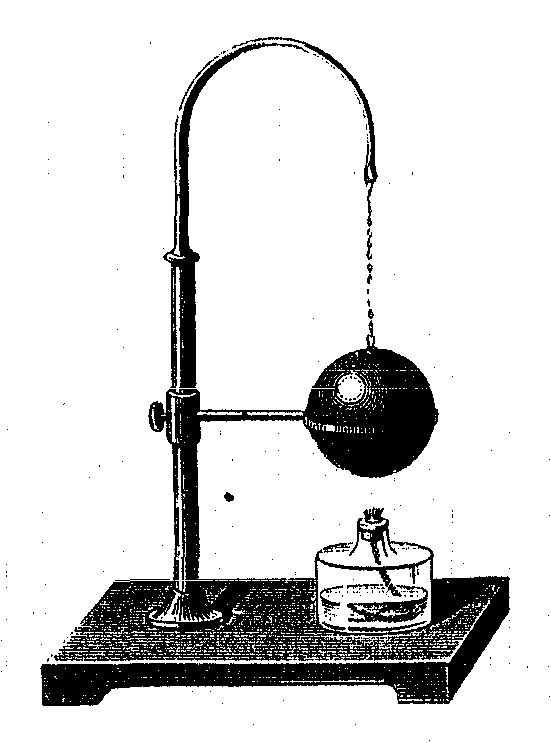
\includegraphics[width=\columnwidth]{img/anello.png}

{\tiny Anello di Gravesande}\pause
\end{figure}
\end{column}
\end{columns}


~

Esiste una relazione tra $ \lambda $ e $ \alpha $:
\begin{center}
$ \alpha = 3 \lambda $
\end{center}\pause

~

Leggi del tutto simili descrivono la dilatazione volumica dei liquidi.
\end{frame}

\begin{frame}
\frametitle{Esempio}
\begin{columns}
\begin{column}{0.7\textwidth}
\begin{exampleblock}{Temperatura massima misurabile}
{\small Un termometro a mercurio ($ \alpha = 1,8 \times 10^{-4} \, K^{-1} $) è composto da una colonnina di vetro (sezione interna di $ 0,10 \, mm^2 $ e altezza di $ 1,25 \, m $) e da un bulbo di volume $ V_0 = 1,0 \times 10^{-6} \, m^3  $.
\begin{itemize}
  \item Sapendo che alla temperatura di $ 0 \, ^\circ C $ il mercurio occupa interamente il bulbo ma non la colonnina, calcola la massima temperatura misurabile dal termometro.
\end{itemize}}
\end{exampleblock}
\end{column}
\begin{column}{0.2\textwidth}
\begin{figure}
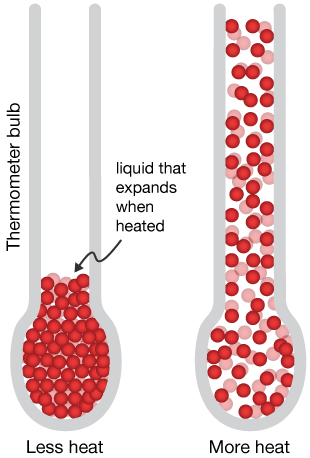
\includegraphics[width=\columnwidth]{img/dilatazionetermica.png}
\end{figure}
\end{column}
\end{columns}
\end{frame}


\section{Gas perfetti}

\begin{frame}
\frametitle{Sistema modello}
Introduciamo un gas in un contenitore sigillato con un pistone mobile per studiarne il comportamento.

~

\begin{columns}
\begin{column}{0.3\textwidth}
\begin{figure}
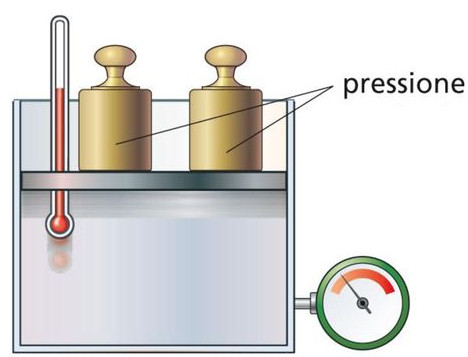
\includegraphics[width=\columnwidth]{img/sistemagas.jpg}
\end{figure}\pause
\end{column}
\begin{column}{0.5\textwidth}
Lo stato del gas è descritto da tre \alert<2>{variabili di stato}:\pause
\begin{itemize}
  \item \alert<3>{volume} $ [m^3 ] $;\pause
  \item \alert<4>{temperatura} $ [ K ] $;\pause
  \item \alert<5>{pressione} $ [ Pa ] $.
\end{itemize}
\end{column}
\end{columns}\pause

~

~

Ogni trasformazione porta il gas da un certo stato ad un altro.
\begin{center}
$ p_0 $, $ V_0 $, $ T_0 $ $ \Longrightarrow $ $ p_1 $, $ V_1 $, $ T_1 $
\end{center}
\end{frame}


\begin{frame}
\frametitle{Trasformazioni}
Tra tutte le trasformazioni che un gas può subire, studieremo quelle:
\begin{itemize}
  \item a \alert<1>{pressione costante} o \emph{isòbare};\pause
  \item a \alert<2>{volume costante} o \emph{isocòre};\pause
  \item a \alert<3>{temperatura costante} o \emph{isoterme}.\pause
\end{itemize}

~

Ognuna di queste trasformazioni è descritta da una legge specifica.\pause

~

\begin{alertblock}{Unità di misura da utilizzare}
La pressione e il volume possono essere espressi con qualsiasi udm appropriata, mentre \emph{la temperatura deve essere in kelvin}.
\end{alertblock}
\end{frame}

\begin{frame}
\frametitle{Trasformazione isòbara}
\begin{block}{Prima legge di Gay-Lussac}
In un gas, volume e temperatura sono direttamente proporzionali.
\begin{center}
$ \dfrac{V}{T} = k $
\end{center}\pause
Se il gas subisce una trasformazione:
\begin{center}
\colorbox{blue!30}{$ \dfrac{V_0}{T_0} = \dfrac{V_1}{T_1} $}
\end{center}
\end{block}
\end{frame}



\begin{frame}
\frametitle{Esempio}
\begin{exampleblock}{Calcolo della temperatura finale}
{\small Un gas perfetto subisce una trasformazione isobara alla pressione costante di $ 1,00 \, atm = 1,01 \times 10^5 \, Pa  $. La temperatura iniziale è di $ 200 \, K $. Durante la trasformazione, il volume del gas raddoppia.

Calcola la temperatura finale.}
\end{exampleblock}
\end{frame}




\begin{frame}
\frametitle{Trasformazione isocòra}
\begin{block}{Seconda legge di Gay-Lussac}
In un gas, pressione e temperatura sono direttamente proporzionali.
\begin{center}
$ \dfrac{p}{T} = k $
\end{center}\pause
Se il gas subisce una trasformazione:
\begin{center}
\colorbox{blue!30}{$ \dfrac{p_0}{T_0} = \dfrac{p_1}{T_1} $}
\end{center}
\end{block}
\end{frame}



\begin{frame}
\frametitle{Trasformazione isoterma}
\begin{block}{Legge di Boyle}
In un gas, pressione e volume sono inversamente proporzionali.
\begin{center}
$ pV = k $
\end{center}\pause
Se il gas subisce una trasformazione:
\begin{center}
\colorbox{blue!30}{$ p_0 V_0 = p_1 V_1 $}
\end{center}
\end{block}\pause

~

Quando un gas rispetta queste leggi, è detto \alert{gas perfetto} (GP).
\end{frame}


\begin{frame}
\frametitle{Piano di Clapeyron}
Le trasformazioni di un gas possono essere rappresentate su un piano volume/pressione.\pause
\begin{columns}
\begin{column}{0.33\textwidth}
\begin{figure}
\begin{tikzpicture}[scale=0.45]
\begin{axis}[
axis x line=bottom,
axis y line=left,
xmin=0, xmax=5,
ymin=0, ymax=4,
xlabel={$V\, [m^3] $},
x label style={at={(axis cs:5,0)},anchor=north},
ylabel={$p\, [Pa] $},
y label style={at={(axis cs:0,4)},rotate=0,anchor=south},
xtick={1,4},
xticklabels={$V_0$,$V_1$},
ytick={2},
yticklabels={$p_1 = p_0 $},
]

\fill [red!40,] (axis cs:1,2) |- (axis cs:4,2) |- (axis cs:1,0) --
            cycle;

        % draw the dashed lines
        % (using two different approaches)
        \addplot [dashed,domain=0:1,samples=2] {2};
        \addplot [dashed,domain=0:4,samples=2] {2};

        \draw [dashed,thin] (axis cs:4,2) -- (axis cs:4,0);
        \draw [dashed,thin] (axis cs:1,2)   -- (axis cs:1,0);
        % now draw the curve
        \draw [
            fleche={0.5:red},
            thick,red              % <-- added
        ] (axis cs:1,2) to [bend right=0]
            % store start and end coordinates
            coordinate [pos=0] (start)
            coordinate [pos=1] (end)
        (axis cs:4,2);

        % draw start and end point
        \fill [radius=2pt,red]
            (start) circle[]
            (end)   circle[];
    \end{axis}
\end{tikzpicture}

{\scriptsize Trasformazione isobara $ p = cost. $}\pause
\end{figure}
\end{column}
\begin{column}{0.33\textwidth}
\begin{figure}
\begin{tikzpicture}[scale=0.45]
\begin{axis}[
axis x line=bottom,
axis y line=left,
xmin=0, xmax=5,
ymin=0, ymax=4,
xlabel={$V\, [m^3] $},
x label style={at={(axis cs:5,0)},anchor=north},
ylabel={$p\, [Pa] $},
y label style={at={(axis cs:0,4)},rotate=0,anchor=south},
xtick={3},
xticklabels={$V_0$},
ytick={1,3},
yticklabels={$p_0$,$p_1 $},
]


% draw the dashed lines
% (using two different approaches)
\draw [dashed,thin] (axis cs:0,1) -- (axis cs:3,1);
\draw [dashed,thin] (axis cs:0,3)   -- (axis cs:3,3);
\draw [dashed,thin] (axis cs:3,0)   -- (axis cs:3,1);

% now draw the curve
\draw [fleche={0.5:red},thick,red] 
  (axis cs:3,1) to [bend right=0]
     % store start and end coordinates
     coordinate [pos=0] (start)
     coordinate [pos=1] (end)
  (axis cs:3,3);

% draw start and end point
\fill [radius=2pt,red] (start) circle[] (end) circle[];
\end{axis}
\end{tikzpicture}

{\scriptsize Trasformazione isocora $ V = cost. $}\pause
\end{figure}
\end{column}
\begin{column}{0.33\textwidth}
\begin{figure}
\begin{tikzpicture}[scale=0.45]
\begin{axis}[
axis x line=bottom,
axis y line=left,
xmin=0, xmax=5,
ymin=0, ymax=6,
xlabel={$V\, [m^3] $},
x label style={at={(axis cs:5,0)},anchor=north},
ylabel={$p\, [Pa] $},
y label style={at={(axis cs:0,6)},rotate=0,anchor=south},
xtick={1,3},
xticklabels={$V_0$,$V_1$},
ytick={1.5,4},
yticklabels={$p_1$,$p_0$},
]

        % fill the area below the curve
        % (draw it first, so it is below everything else)
        \fill [
            red!40,
        ]
            (axis cs:1,4) to [bend right=20]
            (axis cs:3,1.5) |-
            (axis cs:1,\pgfkeysvalueof{/pgfplots/ymin}) |-
            cycle
        ;

        % draw the dashed lines
        % (using two different approaches)
        \addplot [dashed,domain=0:1,samples=2] {4};
        \addplot [dashed,domain=0:3,samples=2] {1.5};

        \draw [dashed,thin] (axis cs:3,1.5) -- (axis cs:3,0);
        \draw [dashed,thin] (axis cs:1,4)   -- (axis cs:1,0);

        % now draw the curve
        \draw [
            fleche={0.5:red},
            thick,red              % <-- added
        ] (axis cs:1,4) to [bend right=20]
            % store start and end coordinates
            coordinate [pos=0] (start)
            coordinate [pos=1] (end)
        (axis cs:3,1.5);

        % draw start and end point
        \fill [radius=2pt,red]
            (start) circle[]
            (end)   circle[];
\end{axis}
\end{tikzpicture}

{\scriptsize Trasformazione isoterma $ pV = cost. $}
\end{figure}
\end{column}
\end{columns}
\end{frame}



\begin{frame}
\frametitle{Equazione di stato del gas perfetto (1)}
\begin{columns}
\begin{column}{0.3\textwidth}
\begin{center}
Isòbara

~

$ \dfrac{V_0}{T_0} = \dfrac{V_1}{T_1} $
\end{center}
\end{column}
\begin{column}{0.3\textwidth}
\begin{center}
Isocòra

~

$ \dfrac{p_0}{T_0} = \dfrac{p_1}{T_1} $
\end{center}
\end{column}
\begin{column}{0.3\textwidth}
\begin{center}
Isoterma

~

$ \textcolor{white}{\dfrac{a}{b}}p_0 V_0 = p_1 V_1 \textcolor{white}{\dfrac{a}{b}}$
\end{center}
\end{column}
\end{columns}\pause

~

~

Possiamo sintetizzare le leggi precedenti con:
\begin{center}
\colorbox{blue!30}{$ \dfrac{p_0 V_0}{T_0} = \dfrac{p_1 V_1}{T_1} $}
\end{center}\pause
Di volta in volta potremo semplificare la quantità che rimane costante durante la trasformazione, ottenendo le leggi precedenti.
\end{frame}


\begin{frame}
\frametitle{Esempio}
\begin{exampleblock}{Trasformazione isocora}
{\small Una bombola contiene idrogeno alla pressione di $ 5,0 \times 10^5 \, Pa $ quando il gas si trova alla temperatura di $ 16 \, ^\circ C $. Successivamente, il manometro della bombola indica una pressione di $ 5,5 \times 10^5 \, Pa $.
\begin{itemize}
  \item Qual è ora la temperatura del gas?
\end{itemize}
}
\end{exampleblock}\pause

~

Il volume è costante ($ V_0 = V_1 $), quindi:
\begin{center}
$ \dfrac{p_0 \cancel{V_0}}{T_0} = \dfrac{p_1 \cancel{V_1}}{T_1} ~~~~\pause \Longrightarrow  ~~~~ \dfrac{p_0}{T_0} = \dfrac{p_1}{T_1}~~~~\pause \Longrightarrow  ~~~~ T_1 = \dfrac{p_1 T_0}{p_0} $
\end{center}\pause
Convertiamo la temperatura in kelvin e calcoliamo:
\begin{center}
$ T_1 = \dfrac{(5,5 \times 10^5 \, Pa) \cdot (289 \, K)}{5,0 \times 10^5 \, Pa} =\pause 318 \, K = 45 \, ^\circ C$
\end{center}
\end{frame}



\begin{frame}
\frametitle{Mole e numero di Avogadro}
Vogliamo anche valutare quante particelle (atomi o molecole) sono contenute in una certa massa di gas (o altro materiale).\pause

~

Introduciamo la \alert<2->{mole}, per misurare la \alert<2>{quantità di sostanza}.\pause

~

Una mole di sostanza:
\begin{itemize}
  \item ha massa in grammi \alert<3>{numericamente uguale alla massa atomica/molecolare};\pause
  \item contiene sempre $ N_A = $ \alert<4>{numero di Avogadro = $ 6,022 \times 10^{23} $} particelle.
\end{itemize}
\end{frame}

\begin{frame}
\frametitle{Esempio}
\begin{exampleblock}{Dalla massa alle moli}
{\small Quante moli di acido solforico $ H_2SO_4 $ corrispondono a $ 0,23 \, kg $?}
\end{exampleblock}\pause

~

Calcoliamo la massa molecolare dell'acido solforico:
\begin{center}
$ 2 \cdot (1,00) + (32,06) + 4 \cdot (15,99) = 98,02 \, u.m.a.$
\end{center}
Una mole di acido solforico ha quindi massa $ 98,02 \, g $.{\pause} Proporzione:
\begin{center}
$ \dfrac{1 mol}{98,02 \, g} = \dfrac{x \, mol}{230 \, g} \pause ~~~~~~~ \Longrightarrow ~~~~~~~ x = \dfrac{230\, g}{98,02 \, g} \, mol = 2,35 \, mol $
\end{center}
\end{frame}

\begin{frame}
\frametitle{Equazione di stato del gas perfetto (2)}
Possiamo intuire che, a pressione e temperatura costanti, \alert<1>{il volume occupato di un gas è direttamente proporzionale al numero di moli} $ n $ di sostanza che lo compongono.\pause

~

Esprimiamo allora l'equazione del GP in funzione del numero di moli $ n $:
\begin{center}
$ \dfrac{p_0 V_0}{T_0} = k \Longrightarrow $ \colorbox{blue!30}{$ pV = nRT $}
\end{center}
$ R = $ costante dei gas perfetti = $ 8,314 \, \dfrac{J}{mol \cdot K} $
\end{frame}



\begin{frame}
\frametitle{Equazione di stato del gas perfetto (3)}
A volte ci troveremo a trattare un gas in termini del numero di particelle che lo compongono.\pause

~

Riformuliamo un'ultima volta l'equazione del GP in funzione del numero di particelle $ N $:
\begin{center}
\colorbox{blue!30}{$ pV = Nk_B T $}
\end{center}
$ k_B = $ costante di Boltzmann = $ 1,381 \times 10^{-23} \, \dfrac{J}{K} $
\end{frame}



\begin{frame}
\frametitle{Esempio}
\begin{exampleblock}{Trovare le moli conoscendo le variabili di stato}
{\small Un palloncino di elio perfettamente sferico ha un raggio di $ 15,0 \, cm $. Al suo interno la pressione è di $ 1,05 \times 10^5 \, Pa $ e la temperatura è di $ 28,0 \, ^\circ C $.
\begin{itemize}
  \item Quante moli di elio sono contenute nel palloncino?
\end{itemize}}
\end{exampleblock}
\end{frame}


\section{Calore}

\begin{frame}
\frametitle{Passaggio di calore}
\begin{block}{Calore}
Il calore $ Q $ è quella quantità che fluisce da un corpo ad un altro quando c'è differenza di temperatura.\pause

~

Come vedremo, si misura in \emph{joule}.
\end{block}
\end{frame}

\begin{frame}
\frametitle{L'esperimento di Joule}
Per scaldare un corpo possiamo:
\begin{itemize}
  \item porlo a contatto con un corpo più caldo;\pause
  \item applicare una forza che compie lavoro.\pause
\end{itemize}

~

Nel 1847 James Prescott Joule riuscì a calcolare quanto \alert<3>{lavoro meccanico} è necessario per aumentare di $ 1\, K $ la temperatura di $ 1 \, kg $ di acqua.\pause

~

Riuscì così a calcolare l'\alert<4>{equivalente meccanico del calore}.
\end{frame}

\begin{frame}
\frametitle{Il mulinello di Joule}

\begin{columns}
\begin{column}{0.5\textwidth}
\begin{figure}
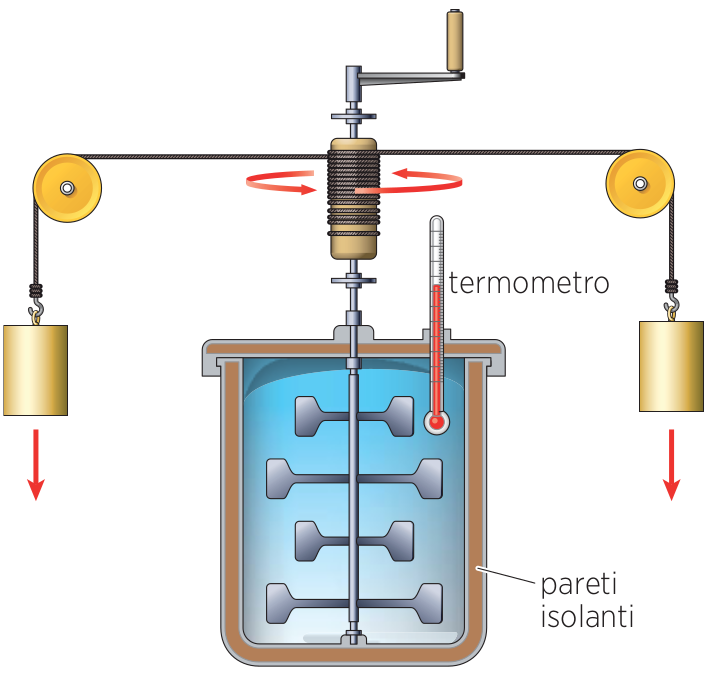
\includegraphics[width=\columnwidth]{img/mulinellojoule.png}
\end{figure}
\end{column}
\begin{column}{0.4\textwidth}\pause

~

~


Possiamo calcolare il lavoro fatto dalla forza peso, che viene trasferito all'acqua mediante le palette, fino a che la temperatura non aumenta di $ 1 \, K $.
\end{column}
\end{columns}
\end{frame}

\begin{frame}
\frametitle{Risultati dell'esperimento}
\begin{enumerate}
  \item Per aumentare di $ 1 \, K $ la temperatura di $ 1 \, kg $ di acqua serve un lavoro di $ 4186 \, J $.\pause
  \item Generalizzando, \alert{calore e lavoro sono modi per trasferire energia da un corpo ad un altro}.
\end{enumerate}

\begin{figure}
\visible<2>{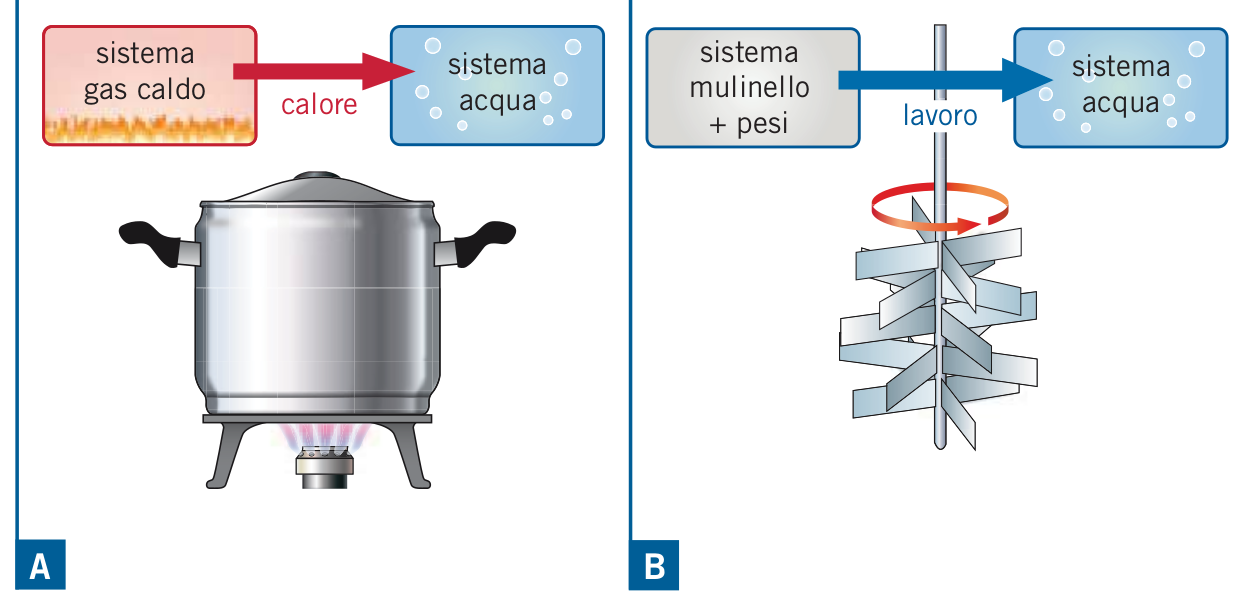
\includegraphics[width=.8\columnwidth]{img/calorelavoro.png}}
\end{figure}
\end{frame}


\begin{frame}
\frametitle{Il calore}
\begin{block}{Calore}
Il calore $ Q $ è una variazione di energia, e pertanto si misura in \emph{joule}.
\end{block}\pause

Per riscaldare un corpo bisogna fornirgli energia. Ciò può avvenire grazie a un flusso di calore (da un corpo più caldo) o al lavoro (compiuto da una forza).\pause

~

Calore e lavoro sono, quindi, \alert{energia in transito}.\pause

~

Dopo che è stata trasmessa mediante calore o lavoro, l’energia
diventa \alert{energia interna} ($ U $).

\end{frame}

\section{Calorimetria}


\begin{frame}
\frametitle{Legge fondamentale della calorimetria}
Possiamo intuire che la quantità di calore da fornire/sottrarre ad un corpo per scaldarlo/raffreddarlo:
\begin{itemize}
  \item \alert<1>{dipende dal materiale} di cui il corpo è fatto;\pause
  \item è \alert<2>{direttamente proporzionale alla sua massa};\pause
  \item è \alert<3>{direttamente proporzionale alla variazione di temperatura}.\pause
\end{itemize}

~

In formula:
\begin{center}
\colorbox{blue!30}{$ Q = c  m  \Delta T $}
\end{center}

\begin{columns}
\begin{column}{0.45\textwidth}
$ c = $ calore specifico $ \left[ \dfrac{J}{kg \cdot K} \right] $
\end{column}
\begin{column}{0.45\textwidth}
\visible<5>{$ c_{H_2O} = 4,186 \times 10^3 \, \dfrac{J}{kg \cdot K} $}
\end{column}
\end{columns}
\end{frame}


\begin{frame}
\frametitle{Esempio}
\begin{exampleblock}{Temperatura raggiunta}
{\small Un cubo di alluminio $\left( c = 8,80 \times 10^2 \, \frac{J}{kg \cdot K} \right)$ di massa $ 2,74 \, kg $ riceve una quantità di calore pari a $ Q = 1,74 \times 10^4 \, J $.
\begin{itemize}
  \item Sapendo che inizialmente si trova alla temperatura di $ 22,0 \, ^\circ C $, calcola la temperatura raggiunta dal cubo.
\end{itemize}
}
\end{exampleblock}\pause

~

Partiamo da $ Q = cm\Delta T $ e troviamo la variazione di temperatura:\pause
\begin{center}
$ \Delta T = \dfrac{Q}{cm} = \pause \dfrac{1,74 \times 10^4 \, J}{\left( 8,80 \times 10^2 \, \dfrac{J}{kg \cdot K} \right)\cdot (2,74 \, kg)} = \pause 7,22 \, K $
\end{center}\pause
Raggiungeremo una temperatura di $ (22,0 + 7,22) \, ^\circ C = 29,2 \, ^\circ C $.
\end{frame}

\begin{frame}
\frametitle{La caloria}
\begin{block}{Definizione di caloria}
Una caloria è la quantità di energia necessaria a portare la temperatura di $ 1 \, g $ di acqua da $ 14,5 \, ^\circ C $ a $ 15,5 \, ^\circ C$.
\begin{center}
\colorbox{blue!30}{$ 1 \, cal = 4, 186 \, J $}\pause

~

$ 1 \, kcal = 1 \, Cal = 4186 \, J $
\end{center}
\end{block}
\end{frame}



\begin{frame}
\frametitle{Temperatura di equilibrio (1)}
Se due corpi a temperatura diversa vengono messi a contatto, essi si scambiano calore.\pause

~

Sapendo che \alert<2>{il calore ceduto dal più caldo viene ricevuto dal più freddo}, calcoliamo la temperatura di equilibrio raggiunta dal sistema.
\begin{center}
$ Q_1 + Q_2 = 0 $\pause

~

$ c_1 m_1 \Delta T_1 + c_2 m_2 \Delta T_2 = 0 $\pause

~

$ c_1 m_1 (T_e - T_1) + c_2 m_2 (T_e - T_2) = 0 $
\end{center}
\end{frame}



\begin{frame}
\frametitle{Temperatura di equilibrio (2)}
\begin{center}
$ c_1 m_1 T_e - c_1 m_1  T_1 + c_2 m_2 T_e - c_2 m_2 T_2 = 0 $\pause

~

$ c_1 m_1 T_e + c_2 m_2 T_e = c_1 m_1 T_1 + c_2 m_2 T_2 $\pause

~

$ (c_1 m_1 + c_2 m_2) T_e = c_1 m_1 T_1 + c_2 m_2 T_2 $\pause

~

\colorbox{blue!30}{$ T_e = \dfrac{c_1 m_1 T_1 + c_2 m_2 T_2}{c_1 m_1 + c_2 m_2} $}

\end{center}
\end{frame}





\begin{frame}
\frametitle{Propagazione del calore}
Il calore è energia in transito, ma \emph{come} avviene questo passaggio?\pause

Sono possibili tre diverse \alert{modalità di propagazione del calore}:
  \begin{columns}
    \begin{column}{0.33\textwidth}
      \visible<3->{\begin{figure}
        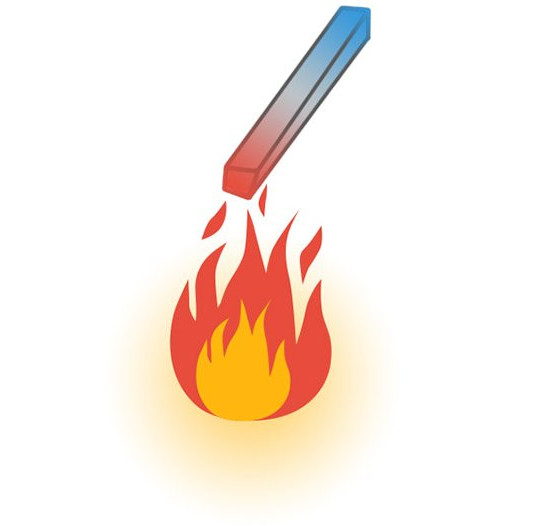
\includegraphics[width=\columnwidth]{img/conduzione.jpg}
      \end{figure}
      \alert<3->{Conduzione}, senza spostamento di materia.}
    \end{column}
    \begin{column}{0.33\textwidth}
      \visible<4->{\begin{figure}
        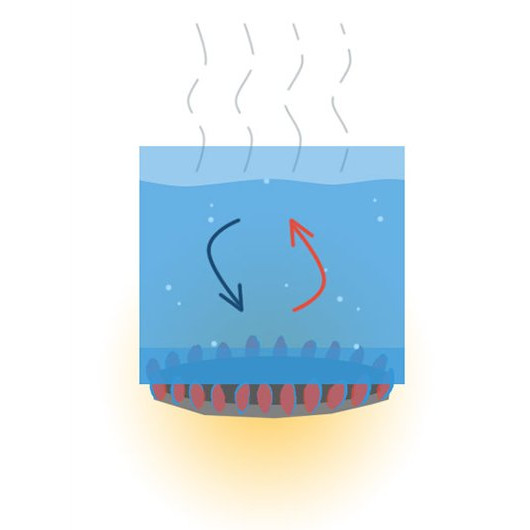
\includegraphics[width=\columnwidth]{img/convezione.jpg}
      \end{figure}
      \alert<4->{Convezione}, mediante correnti che trasportano materia.}
    \end{column}
    \begin{column}{0.33\textwidth}
      \visible<5>{\begin{figure}
        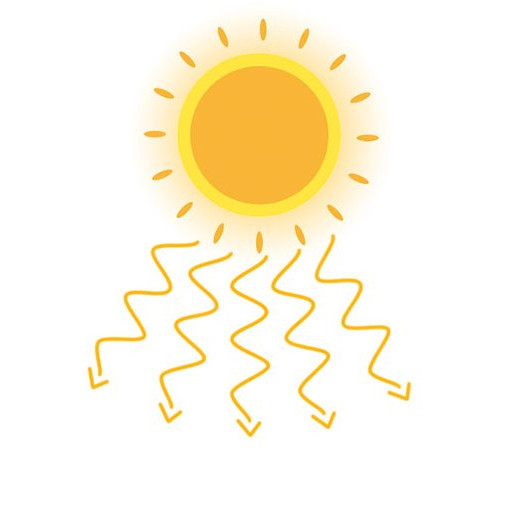
\includegraphics[width=\columnwidth]{img/irraggiamento.jpg}
      \end{figure}
      \alert<5->{Irraggiamento}, mediante onde elettromagnetiche.}
    \end{column}
  \end{columns}
\end{frame}




\begin{frame}
\frametitle{Esempi macroscopici di convezione}
\begin{figure}
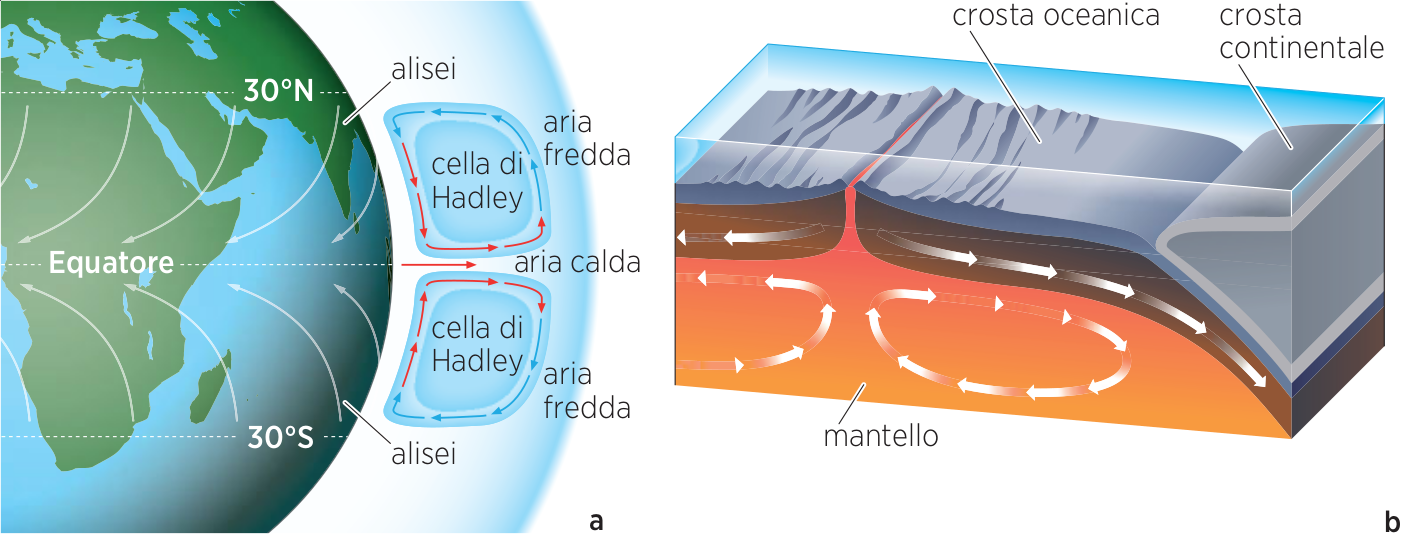
\includegraphics[width=\columnwidth]{img/convezione1.png}
\end{figure}
\end{frame}


\section{Materia}



\begin{frame}
\frametitle{Moto browniano}
\begin{columns}
\begin{column}{0.2\textwidth}
\visible<1->{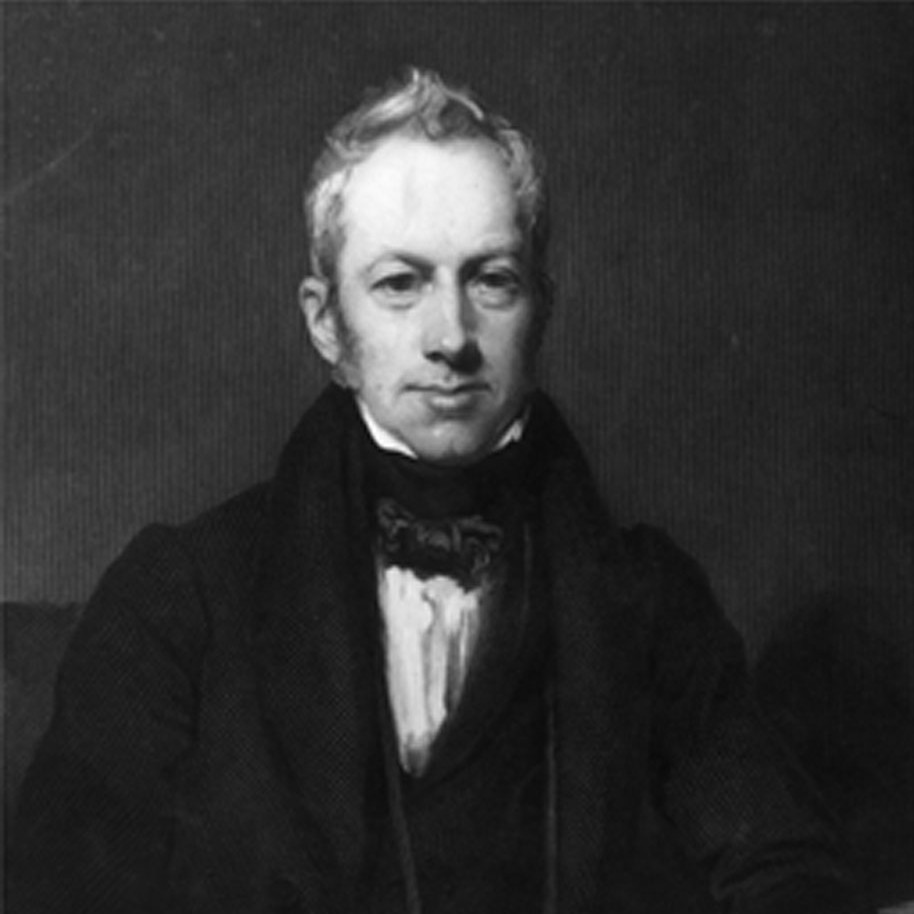
\includegraphics[width=\columnwidth]{img/brown.jpg}}
~
\visible<2->{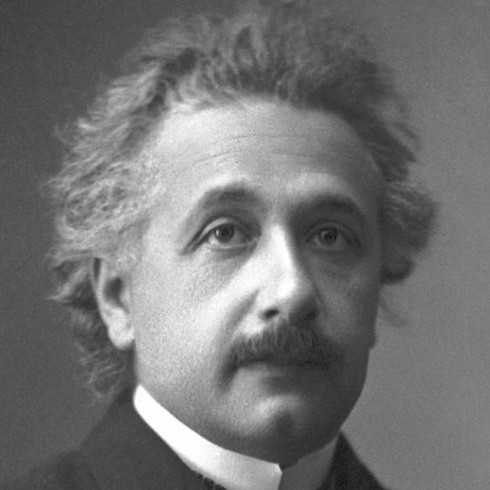
\includegraphics[width=\columnwidth]{img/einstein2.jpg}}
~
\visible<3->{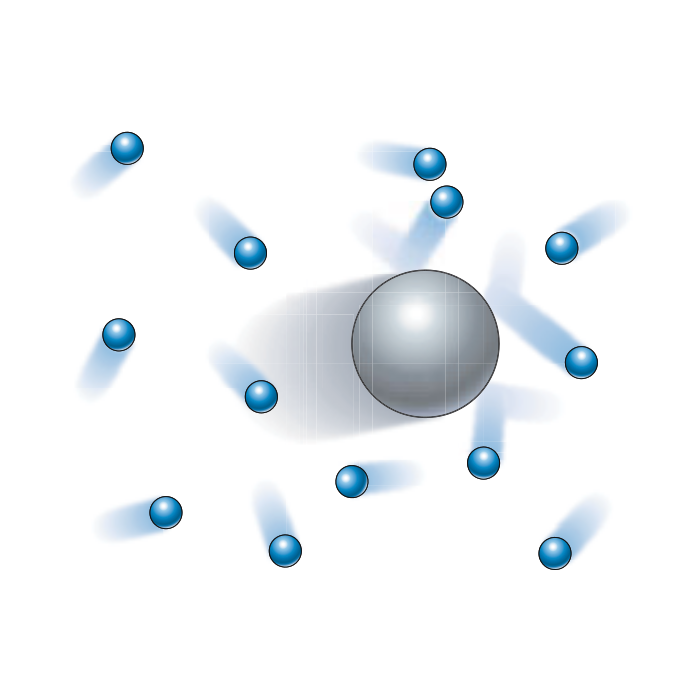
\includegraphics[width=\columnwidth]{img/motobrowniano.png}}
\end{column}
\begin{column}{0.6\textwidth}
\begin{itemize}
\item<1-> 1827: il botanico Brown osserva che un granello di polline sospeso in acqua si muove a zig-zag, in modo irregolare.

~

\item<2-> 1905: Einstein propone che i granelli si muovano così perché continuamente colpiti dalle particelle d'acqua;

~

\item<3-> l'ipotesi di Einstein è una ulteriore conferma della teoria atomica della materia.
\begin{center}
\href{video/Brown.mp4}{\beamergotobutton{Video: Moto browniano}}
\end{center}
\end{itemize}
\end{column}
\end{columns}
\end{frame}





\begin{frame}
\frametitle{Lavorare con molte particelle}
La teoria atomica della materia ci pone di fronte ad un \alert<1>{enorme numero di particelle}, rendendo impossibile l'applicazione ad ognuna di esse la meccanica newtoniana.\pause

~

Ricorreremo pertanto alla statistica e considereremo le \alert{proprietà medie} delle particelle del gas.
\end{frame}


\begin{frame}
\frametitle{Teoria cinetica dei gas (1)}
Presentiamo il modello microscopico per i gas perfetti, che permette di trovare un \alert{collegamento tra i fenomeni termici e le leggi della meccanica}, seguite dalle particelle nel loro moto.\pause

~

~

\centering
\begin{tabular}{p{0.4\textwidth}p{0.1\textwidth}p{0.4\textwidth}}
\textbf{Condizioni} & per le & \textbf{ipotesi sulle particelle} \\\rule{0pt}{5ex}\pause
\hspace*{-1.4mm}1.~Le dimensioni delle particelle sono molto minori del loro cammino libero medio & ~$ \longrightarrow  $ & Le particelle sono intese come punti materiali di uguale massa \\\rule{0pt}{5ex}\pause
\hspace*{-1.4mm}2.~In una mole di gas ci sono $ 6,022 \times 10^{23} $ particelle & ~$ \longrightarrow  $ & Possiamo trascurare l'effetto del singolo movimento\\
\end{tabular}
\end{frame}


\begin{frame}
\frametitle{Teoria cinetica dei gas (2)}
\centering
\begin{tabular}{p{0.4\textwidth}p{0.1\textwidth}p{0.4\textwidth}}
\textbf{Condizioni} & per le & \textbf{ipotesi sulle particelle} \\\rule{0pt}{5ex}
\hspace*{-4mm}3.~Si conservano energia e quantità di moto delle particelle & ~$ \longrightarrow  $ & Le particelle compiono urti elastici tra loro e con il recipiente \\\rule{0pt}{5ex}\pause
\hspace*{-1.4mm}4.~Le particelle sono sufficientemente lontane da poter trascurare le interazioni a distanza & ~$ \longrightarrow  $ & Tra un urto e l'altro le particelle si muovono di moto rettilineo uniforme \\\rule{0pt}{5ex}\pause
\hspace*{-1.4mm}5.~Le particelle si muovono in modo casuale & ~$ \longrightarrow  $ & Non ci sono direzioni di moto privilegiate (ipotesi di \alert{isotropia}) \\
\end{tabular}
\end{frame}



\begin{frame}
\frametitle{La velocità quadratica media}
La grandezza chiave della teoria cinetica dei gas è la velocità delle particelle.\pause

~

Per l'isotropia, se calcolassimo la velocità media delle $ N $ particelle:
\begin{center}
$ \overline{v} = \dfrac{\vec{v_1} + \vec{v_2} + ... + \vec{v_N}}{N} =\pause \dfrac{\sum\limits_{i=1}^N v_i}{N} =\pause 0 $
\end{center}\pause

Ricorriamo allora alla \alert{velocità quadratica media}:
\begin{center}
\colorbox{blue!30}{$ v_{qm} = \sqrt{\dfrac{v_1^2 + v_2^2 + ... + v_N^2}{N}} = \sqrt{\dfrac{\sum v_i^2}{N}} $}
\end{center}
\end{frame}

\begin{frame}
\frametitle{Velocità delle particelle e temperatura}
Definiamo allora l'energia cinetica media delle particelle di un gas:
\begin{center}
$ \overline{K} = \dfrac{1}{2}mv_{qm}^2 $
\end{center}\pause
È possibile dimostrare che \alert{l'energia cinetica delle particelle è legata direttamente alla temperatura assoluta del gas}.
\begin{center}
\colorbox{blue!30}{$ \overline{K} = \dfrac{\ell}{2}k_B T $}
\end{center}
$ \ell = $ numero di gradi di libertà della particella
\begin{itemize}
  \item $ \ell = 3 $ per gas monoatomici
  \item$ \ell = 5 $ per gas biatomici
\end{itemize}
\end{frame}

\begin{frame}
\frametitle{Energia interna di una gas}
Sotto l'ipotesi che le particelle non interagiscono tra loro, possiamo affermare che \alert<1>{le particelle del gas possiedono solo energia cinetica}.\pause

~

Pertanto \alert<2>{l'energia del gas perfetto è la somma delle energie cinetiche} delle particelle che lo compongono.\pause

~

Basta moltiplicare $ \overline{K} $ per il numero di particelle:
\begin{center}
\colorbox{blue!30}{$ U = N\overline{K} = \dfrac{\ell}{2}Nk_B T = \dfrac{\ell}{2}nR T$}
\end{center}
\end{frame}

\begin{frame}
\frametitle{Interpretazione cinetica dello zero assoluto}
Lo zero assoluto corrisponde alla situazione di \alert<1>{perfetta immobilità delle particelle}.\pause

~

Esse hanno $ U = 0 $ e \alert{non possono essere ulteriormente rallentate/raffreddate}.


\begin{figure}\centering
\begin{tikzpicture}[scale=0.4]
\draw [->] (-7,0) -- (7,0);
\draw [->] (0,0) -- (0,7);
\draw [->,dotted] (0,0) -- (0,7);
\node [below] at (7,0) {$ T $};
\node [below] at (0,0) {\tiny $ 0 \, ^\circ C $};
\node [below] at (0,-1) {\tiny $ 273 \, K $};
\node [below] at (-6,0) {\tiny $ -273 \, ^\circ C $};
\node [below] at (-6,-1) {\tiny $ 0 \, K $};
\node [left] at (0,7) {$ U  $};
\draw [thick,red] (-6,0) -- (7,7);
\end{tikzpicture}
\end{figure}
\end{frame}



\section{Stati}



\begin{frame}
\frametitle{Stati della materia}
La materia (composta da atomi, che formano molecole), può presentarsi in tre stati:
\begin{figure}
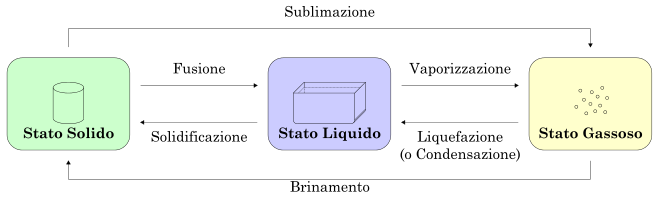
\includegraphics[width=.9\columnwidth]{img/passaggidistato.png}
\end{figure}
\begin{columns}
\begin{column}{0.3\textwidth}
\begin{center}
I solidi hanno volume e forma propria.\\~
\end{center}
\end{column}
\begin{column}{0.3\textwidth}
\begin{center}
I liquidi hanno un volume, ma non una forma propria.\\~
\end{center}
\end{column}
\begin{column}{0.3\textwidth}
\begin{center}
I gas occupano tutto lo spazio del recipiente che li contiene.
\end{center}
\end{column}
\end{columns}
\end{frame}


\begin{frame}
\frametitle{Passaggi di stato}
Durante un passaggio di stato, il calore fornito (sottratto) viene utilizzato per rompere (formare) i legami tra le particelle, e non per aumentare (diminuire) la temperatura della sostanza.
\begin{figure}
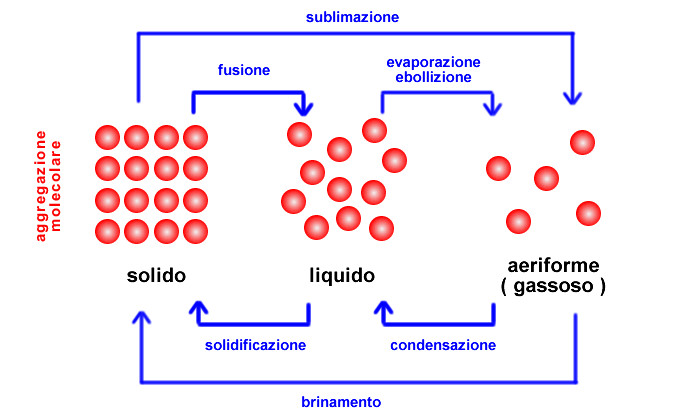
\includegraphics[width=.8\columnwidth]{img/aggregazione.jpg}
\end{figure}
\end{frame}



\begin{frame}
\frametitle{Grafico calore/temperatura per l'acqua}
A seguito di quanto detto, possiamo verificare sperimentalmente che \alert{durante un passaggio di stato la temperatura della sostanza rimane costante}.\pause

\begin{figure}
\begin{tikzpicture}[scale=0.3]
\draw [->] (0,0) -- (21,0);
\draw [->] (0,0) -- (0,12);
\node [below] at (21,0) {$ Q $};
\node [left] at (0,12) {$ T $};
\draw [dashed] (0,5) -- (4,5);
\node [left] at (0,5) {\footnotesize $ 0 \, ^\circ C $};
\node [left] at (0,9) {\footnotesize $ 100 \, ^\circ C $};
\draw [dashed] (0,9) -- (12,9);
\draw [thick,orange] (0,2) -- (4,5) -- (8,5) -- (12,9) -- (17,9) -- (20,11);
\node [above,red] at (6,5) {\tiny fusione};
\node [below,blue] at (6,5) {\tiny solidificazione};
\node [above,red] at (14.5,9) {\tiny ebollizione};
\node [below,blue] at (14.5,9) {\tiny condensazione};
\node [below,orange,rotate=45] at (10,7) {\tiny acqua};
\node [below,orange,rotate=37] at (2,3.5) {\tiny ghiaccio};
\node [below,orange,rotate=34] at (18.8,10) {\tiny vapore};
\end{tikzpicture}
\end{figure}
\end{frame}


\begin{frame}
\frametitle{Un problema}
Durante un passaggio di stato, avremo che:
\begin{itemize}
  \item $ \Delta T = 0 $;\pause
  \item $ Q > 0 $ per fusione ed ebollizione, $ Q<0 $ per solidificazione e condensazione.\pause
\end{itemize}

~

La legge $ Q = cm\Delta T $ non è utilizzabile!
\end{frame}


\begin{frame}
\frametitle{Leggi per i passaggi di stato}
Per \alert<1>{vaporizzazione e condensazione} vale:
\begin{center}
\colorbox{blue!30}{$ Q = \pm L_v m $}


$ L_v = $ calore latente di vaporizzazione $ \left[ \dfrac{J}{kg} \right] $
\end{center}\pause

~

Per \alert<2>{fusione e solidificazione} vale:
\begin{center}
\colorbox{blue!30}{$ Q = \pm L_f m $}


$ L_f = $ calore latente di fusione $ \left[ \dfrac{J}{kg} \right] $
\end{center}
\end{frame}


\begin{frame}
\frametitle{Esempio}
\begin{exampleblock}{Stato finale dopo un riscaldamento}
{\small Indica lo stato (solido, liquido o aeriforme) e la temperatura di $ 1,00 \times 10^{-1} \, kg  $ di acqua, inizialmente alla temperatura di $ 278 \, K $, che ricevono $ 3,20 \times 10^5 \, J  $ di calore.

~

Dati: $ c_{vapore \, acqueo} = 1940 \, \frac{J}{kg\cdot K} $, $ L_v = 2200 \times 10^3 \, \frac{J}{kg} $.}
\end{exampleblock}
\end{frame}



\begin{frame}
\frametitle{Stati della materia e pressione}
Finora abbiamo ipotizzato di \alert<1>{mantenere la pressione costante}.\pause

~

Tuttavia, gli stati della materia \alert<2>{dipendono dalla temperatura e dalla pressione}.

\begin{center}
\href{video/Acqua.mp4}{\beamergotobutton{Video: Ebollizione dell'acqua a temperatura ambiente}}
\end{center}
\end{frame}


\begin{frame}
\frametitle{Diagramma di fase}
\begin{figure}
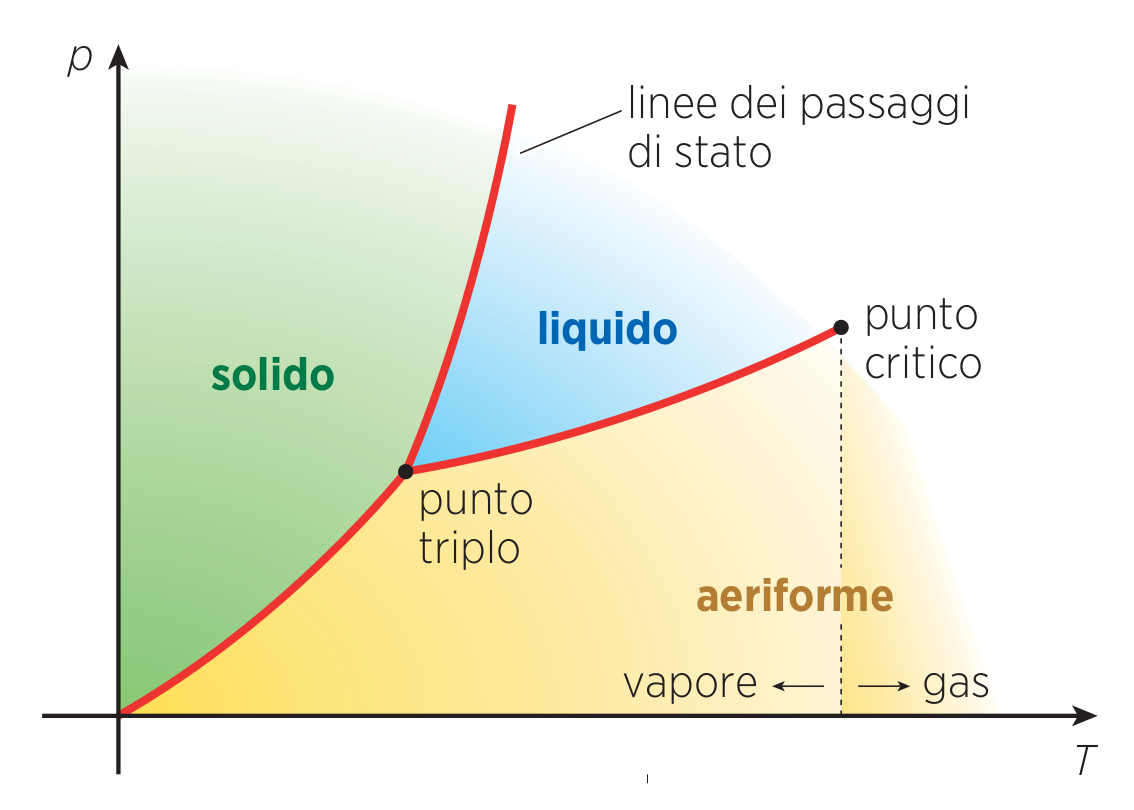
\includegraphics[width=.9\columnwidth]{img/diagrammadifase.png}
\end{figure}
\end{frame}


\begin{frame}
\frametitle{Diagramma di fase dell'acqua}
\begin{figure}
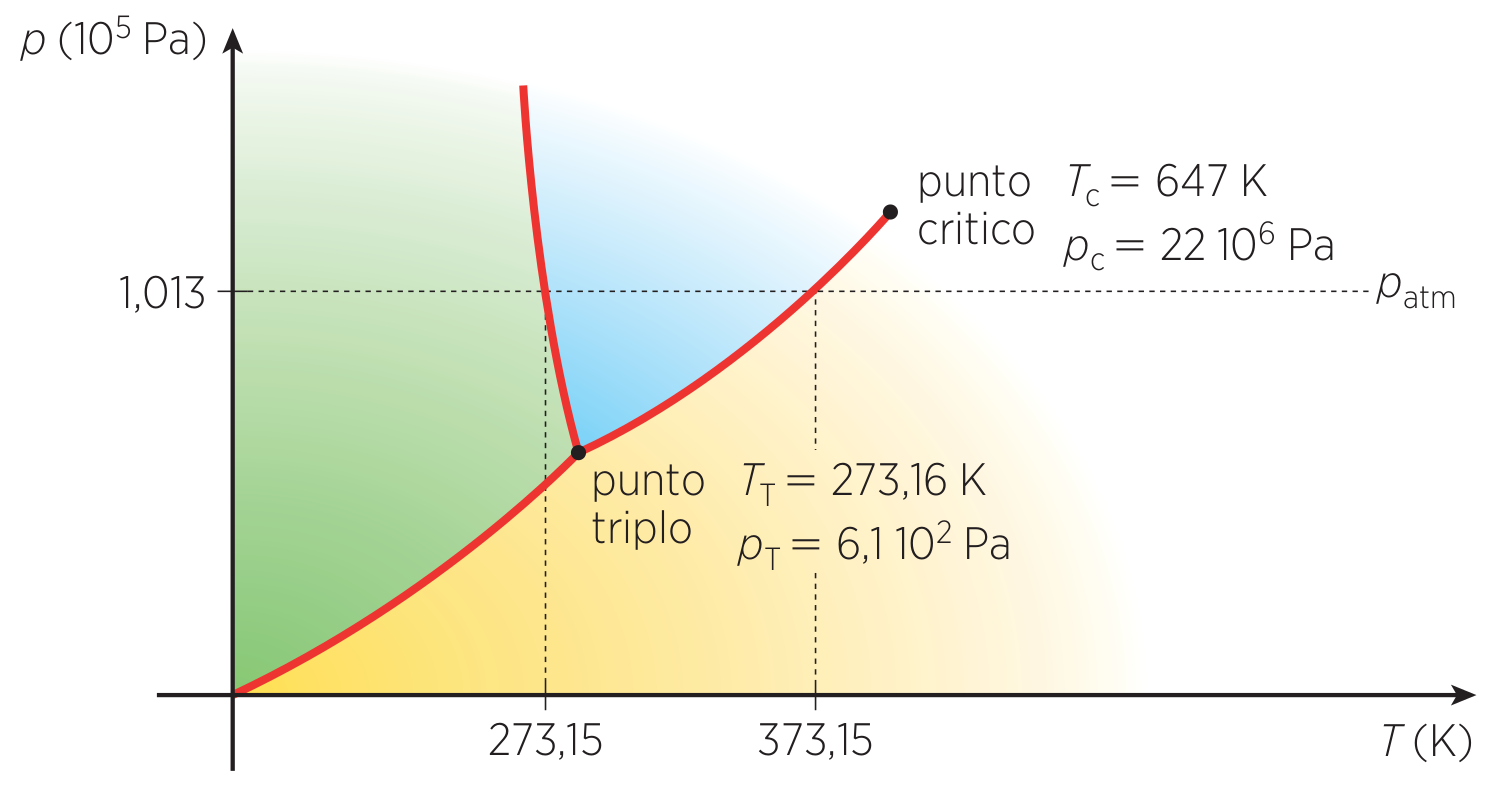
\includegraphics[width=\columnwidth]{img/diagrammadifase2.png}
\end{figure}
\end{frame}



\end{document}
